\section{Results}


In Table~\ref{tab:results}, we showcase the optimal results obtained by our models. To evaluate their performance, we furnish information about the optimal parameter combinations, accompanied by key metrics:

\begin{itemize}
    \item \textbf{Accuracy:} measure of the overall correctness of a classification model. It is calculated as the ratio of correctly predicted instances to the total instances.
    
    \item \textbf{Precision:} measure of the accuracy of the positive predictions made by a classification model. It calculates the ratio of correctly predicted positive observations to the total predicted positives.
    
    \item \textbf{Recall:} measure of the ability of a classification model to capture and correctly identify all the relevant instances. It calculates the ratio of correctly predicted positive observations to the total actual positives.
    
    \item \textbf{F1 Score:} harmonic mean of precision and recall, offering a balanced assessment that considers both false positives and false negatives.
    
\end{itemize}

In all these metrics we considered as positive label the "positive" rating. This comprehensive set of metrics offers a well-rounded assessment of our model's performance across various dimensions. Table~\ref{tab:results} summarize for each possible combination of embedder and classifier the best model obtained with the grid search.



\begin{table}[h]
    \centering
    \begin{tabular}{cccccc}
    \textbf{Model} & \textbf{Parameters}                                                                                & \textbf{Accuracy} & \textbf{Precision} & \textbf{Recall} & \textbf{F1 Score} \\ \hline
    T + LR    & \begin{tabular}[c]{@{}c@{}}max\_features: 10000\\ C: 1\\ penalty: l2\end{tabular}                  & 0.88              & 0.875              & 0.889           & 0.881             \\ \hline
    T + SVM   & \begin{tabular}[c]{@{}c@{}}max\_features: 10000\\ C: 10\\ gamma: scale\\ kernel: rbf\end{tabular}  & 0.878             & 0.883              & 0.871           & 0.877             \\ \hline
    BoW + SVM      & \begin{tabular}[c]{@{}c@{}}max\_features: 10000\\ C: 10\\ gamma: scale\\ kernel: rbf\end{tabular}  & 0.875             & 0.88               & 0.869           & 0.874             \\ \hline
    BoW + LR       & \begin{tabular}[c]{@{}c@{}}max\_features: 10000\\ C: 1\\ penalty: l2\end{tabular}                  & 0.867             & 0.864              & 0.871           & 0.868             \\ \hline
    T + NB    & \begin{tabular}[c]{@{}c@{}}max\_features: 5000\\ alpha: 1\\ fit\_prior: False\end{tabular}         & 0.837             & 0.86               & 0.806           & 0.832             \\ \hline
    BoW + NB       & \begin{tabular}[c]{@{}c@{}}max\_features: 5000\\ alpha: 1\\ fit\_prior: True\end{tabular}          & 0.837             & 0.86               & 0.805           & 0.832             \\ \hline
    W2V + SVM      & \begin{tabular}[c]{@{}c@{}}num\_features: 300\\ C: 10\\ gamma: 1\\ kernel: linear\end{tabular}     & 0.83              & 0.83               & 0.831           & 0.83              \\ \hline
    FT + SVM       & \begin{tabular}[c]{@{}c@{}}num\_features: 1000\\ C: 10\\ gamma: auto\\ kernel: linear\end{tabular} & 0.82              & 0.818              & 0.823           & 0.82              \\ \hline
    W2V + LR       & \begin{tabular}[c]{@{}c@{}}num\_features: 100\\ C: 0.1\\ penalty: l2\end{tabular}                  & 0.807             & 0.809              & 0.804           & 0.806             \\ \hline
    FT + LR        & \begin{tabular}[c]{@{}c@{}}num\_features: 300\\ C: 0.1\\ penalty: l2\end{tabular}                  & 0.806             & 0.807              & 0.804           & 0.805             \\ \hline
    \end{tabular}
    \caption{Best performance for each combination of embedder (T: TF-IDF, BoW: Bag of Words, W2V: Word2Vec, FT: FastText) and classifier (LR: Logistic Regression, SVM, NB: Naive Bayes).}
    \label{tab:results}
\end{table}


The obtained results demonstrate a robust generalization of all our models for this task, employing various techniques. This success can be attributed to the high quality of our pre-processing methods. The optimal approach for such tasks appears to involve a combination of a vector space model and a classification model, choosing between logistic regression and SVM. Despite training on the entire dataset, it appears that the corpus may not be sufficient to provide word embeddings with the necessary information to accurately represent the reviews.

To conclude our analysis, we futher analyze the performance of the best model in order to understand whether the errors are due to one of the general features of the reviews, or if it is mostly due to randomness.

To accomplish this, we computed the same distributions as presented in Section~\ref{sec:eda}, with a focus on highlighting the segment of data that has been misclassified. Figures~\ref{fig:pred_distro_ratings} and \ref{fig:pred_distro_length} depict the expected patterns from a well-generalizing model that exhibits no bias stemming from certain features.

Observing Figure~\ref{fig:pred_distro_ratings} and \ref{fig:pred_distro_length}, it becomes apparent that the model performs with higher accuracy on more extreme reviews, aligning with expectations and demonstrating proficiency in tasks that involve clear sentiment. However, as the rating approaches neutrality, the accuracy diminishes, indicating a potential need for further training to enhance performance to an even higher level. Importantly, this trend is consistent across reviews of varying lengths, suggesting that the model's performance remains stable and is not significantly influenced by the length of the reviews.

As a final verification step, we presented in Table~\ref{tab:logreg} the words associated with the highest coefficients in the Logistic Regression step. Examining these words allows us to confirm that the model has learned a set of terms that effectively represent either positive or negative sentiment, thereby equipping the model with a robust set of rules for accurately classifying reviews.



\begin{figure}[h]
    \begin{subfigure}{0.5\textwidth}
      \centering
      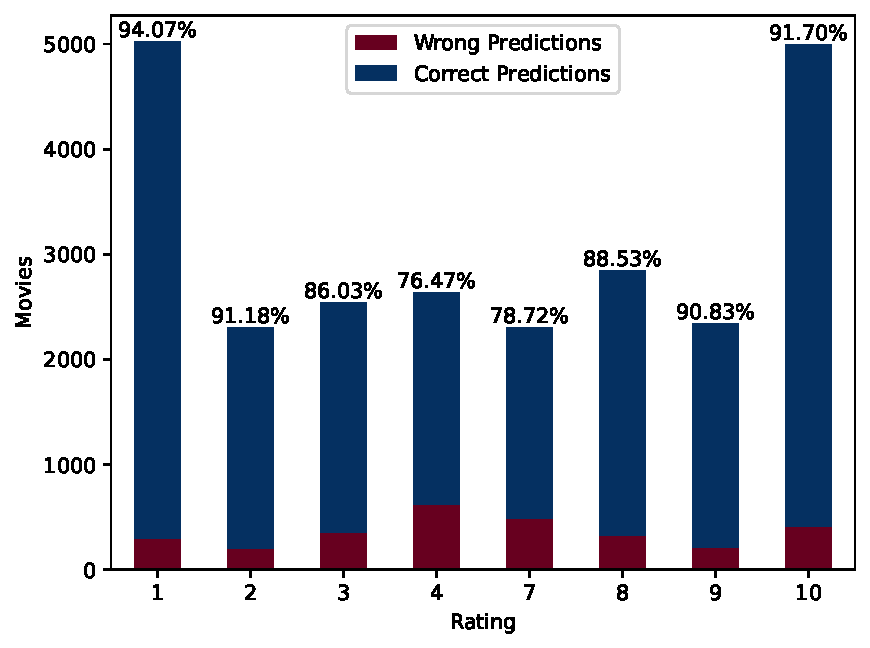
\includegraphics[width=\linewidth]{figures/t_lr_ratings.pdf}
      \caption{Predictions' distribution based on Ratings}
      \label{fig:pred_distro_ratings}
    \end{subfigure}%
    \begin{subfigure}{0.5\textwidth}
      \centering
      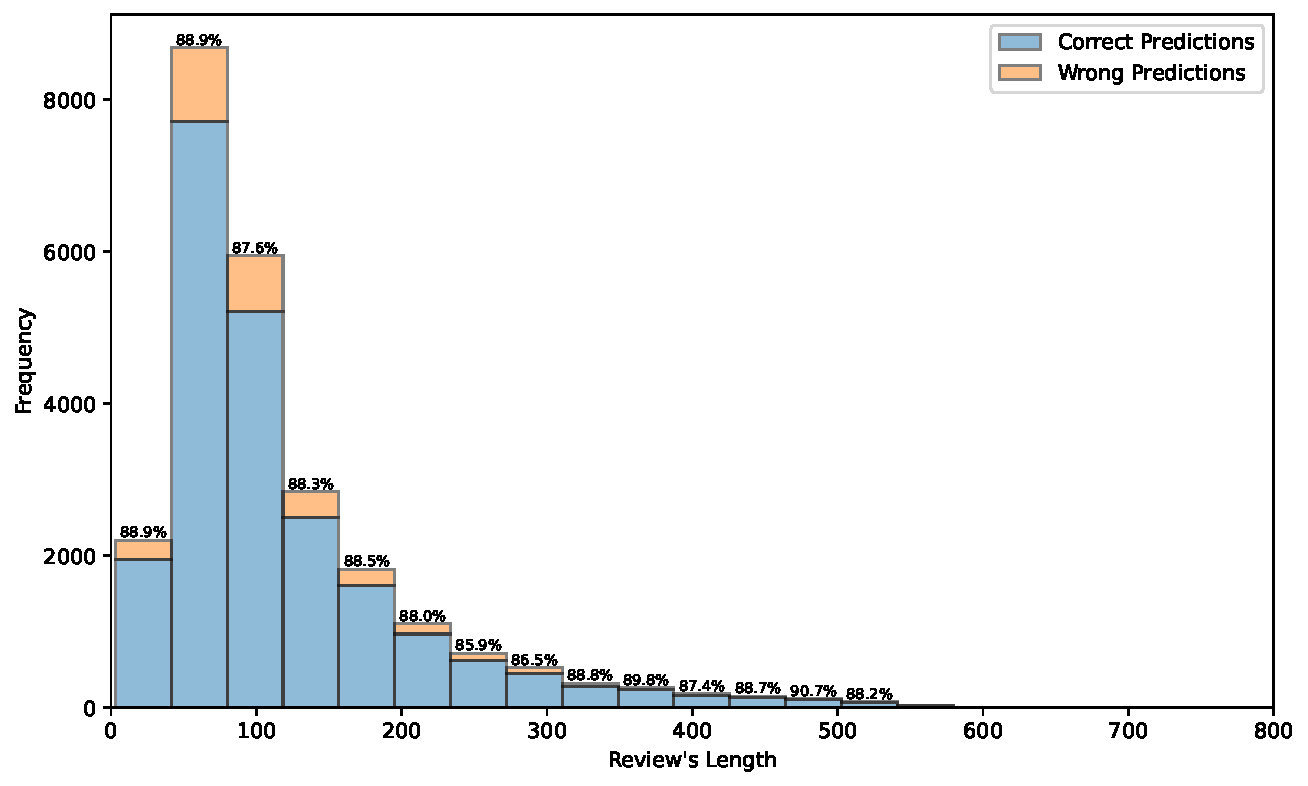
\includegraphics[width=\linewidth]{figures/t_lr_lengths.pdf}
      \caption{Predictions' distribution based on Reviews' length}
      \label{fig:pred_distro_length}
    \end{subfigure}
    \caption{}
  
  \end{figure}



\begin{table}[h]
    \centering
    \begin{tabular}{ccccc}
    \multicolumn{2}{c}{\textbf{Most "Positive" words}} &  & \multicolumn{2}{c}{\textbf{Most "Negative" words}} \\ \cline{1-2} \cline{4-5} 
    \multicolumn{1}{c|}{great}          & 6.519     &  & \multicolumn{1}{c|}{worst}            & -8.950  \\ \cline{1-2} \cline{4-5} 
    \multicolumn{1}{c|}{excellent}      & 5.974     &  & \multicolumn{1}{c|}{bad}              & -7.058  \\ \cline{1-2} \cline{4-5} 
    \multicolumn{1}{c|}{best}           & 4.933     &  & \multicolumn{1}{c|}{waste}            & -6.468  \\ \cline{1-2} \cline{4-5} 
    \multicolumn{1}{c|}{perfect}        & 4.732     &  & \multicolumn{1}{c|}{awful}            & -6.437  \\ \cline{1-2} \cline{4-5} 
    \multicolumn{1}{c|}{wonderful}      & 4.564     &  & \multicolumn{1}{c|}{boring}           & -5.642  \\ \cline{1-2} \cline{4-5} 
    \multicolumn{1}{c|}{amazing}        & 4.018     &  & \multicolumn{1}{c|}{poor}             & -5.177  \\ \cline{1-2} \cline{4-5} 
    \multicolumn{1}{c|}{favorite}       & 4.009     &  & \multicolumn{1}{c|}{nothing}          & -4.819  \\ \cline{1-2} \cline{4-5} 
    \multicolumn{1}{c|}{well}           & 3.824     &  & \multicolumn{1}{c|}{terrible}         & -4.621  \\ \cline{1-2} \cline{4-5} 
    \multicolumn{1}{c|}{loved}          & 3.655     &  & \multicolumn{1}{c|}{worse}            & -4.591  \\ \cline{1-2} \cline{4-5} 
    \multicolumn{1}{c|}{fun}            & 3.523     &  & \multicolumn{1}{c|}{poorly}           & -4.364  \\ \cline{1-2} \cline{4-5} 
    \multicolumn{1}{c|}{enjoyed}        & 3.516     &  & \multicolumn{1}{c|}{horrible}         & -4.283  \\ \cline{1-2} \cline{4-5} 
    \multicolumn{1}{c|}{love}           & 3.488     &  & \multicolumn{1}{c|}{dull}             & -4.186  \\ \cline{1-2} \cline{4-5} 
    \multicolumn{1}{c|}{highly}         & 3.479     &  & \multicolumn{1}{c|}{unfortunately}    & -4.043  \\ \cline{1-2} \cline{4-5} 
    \multicolumn{1}{c|}{today}          & 3.451     &  & \multicolumn{1}{c|}{disappointment}   & -4.043  \\ \cline{1-2} \cline{4-5} 
    \multicolumn{1}{c|}{superb}         & 3.285     &  & \multicolumn{1}{c|}{supposed}         & -3.839  \\ \cline{1-2} \cline{4-5} 
    \multicolumn{1}{c|}{brilliant}      & 3.281     &  & \multicolumn{1}{c|}{annoying}         & -3.791  \\ \cline{1-2} \cline{4-5} 
    \multicolumn{1}{c|}{definitely}     & 3.145     &  & \multicolumn{1}{c|}{disappointing}    & -3.681  \\ \cline{1-2} \cline{4-5} 
    \multicolumn{1}{c|}{enjoyable}      & 3.115     &  & \multicolumn{1}{c|}{ridiculous}       & -3.647  \\ \cline{1-2} \cline{4-5} 
    \multicolumn{1}{c|}{beautiful}      & 2.975     &  & \multicolumn{1}{c|}{fails}            & -3.635  \\ \cline{1-2} \cline{4-5} 
    \multicolumn{1}{c|}{fantastic}      & 2.965     &  & \multicolumn{1}{c|}{script}           & -3.616  \\ \cline{1-2} \cline{4-5} 
    \end{tabular}
    \caption{Words associated to largest coefficient in the Logistic Regression of the T+LR model.}
    \label{tab:logreg}
\end{table}
    





